%!TEX program = xelatex
% 完整编译: xelatex -> bibtex -> xelatex -> xelatex
\documentclass[lang=cn,11pt,a4paper,cite=numbers]{elegantpaper}
\usepackage{xfp}
\usepackage{tikz}

\title{从另一个角度看拉普拉斯变换}
\author{郑晖}
% \institute{}

% \version{0.09}
\date{\zhtoday}

% 本文档命令
\usepackage{array}
\newcommand{\ccr}[1]{\makecell{{\color{#1}\rule{1cm}{1cm}}}}

\begin{document}

\maketitle

\begin{abstract}
拉普拉斯变换可以说是现代工程学中使用最广泛的数学工具,它通过数学变换将微积分方程转化成代数方程,为求解连续空间连续时间的方程提供了可能。但是,一般的教材上一上来就是拉普拉斯变换的数学定义,对于其历史和代表的深刻含义没有任何介绍,导致很多人一直头疼不已。在这项学习报告中,我们尝试一下从不同的角度来看看拉普拉斯变换到底是怎么回事?先从一个人说起:奥列弗·赫维赛德,一位在科学史地位被严重低估的人。
\keywords{拉普拉斯变换}
\end{abstract}

\section{奥列弗·赫维赛德是何许人也}
  奥列弗·赫维赛德(Oliver Heaviside)是维多利亚时期的英国人,出身于极度贫穷的家庭,听力部分残疾,还得过猩红热,从未上过大学,完全靠自学和兴趣掌握了高等科学和数学。
\begin{figure}[!htb]
  \centering
  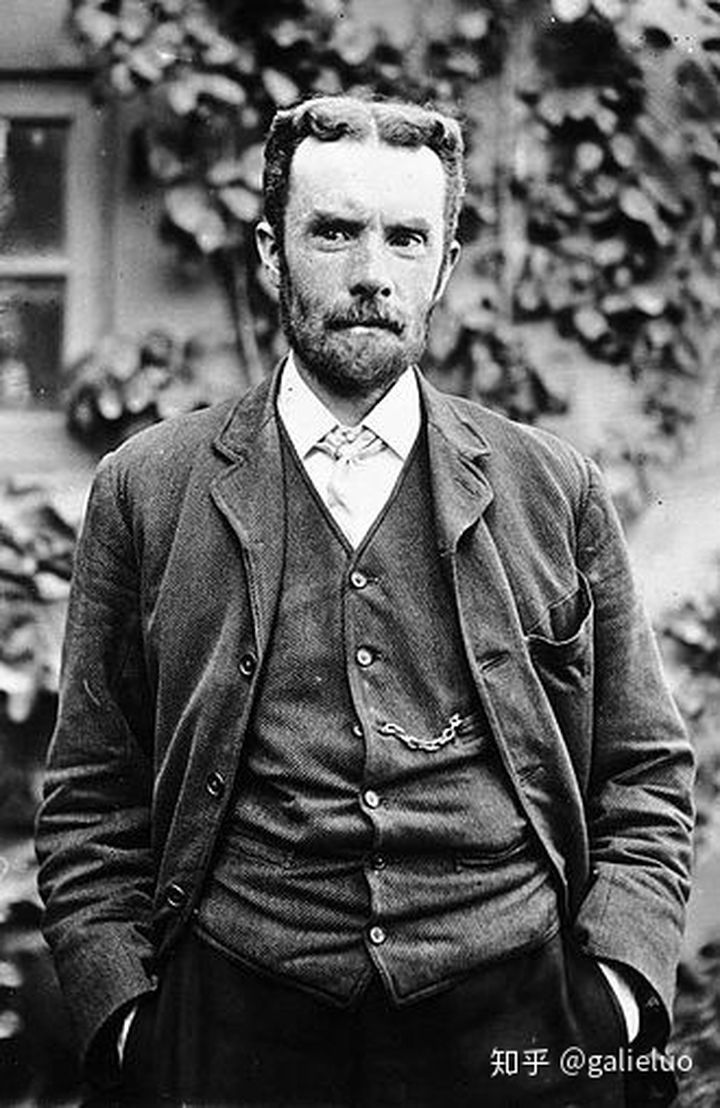
\includegraphics[width=0.4\textwidth]{figs/oliver-heaviside.png}
  \caption{figs:oliver-heaviside}
  \label{figs:oliver-heaviside}
\end{figure}

  很多人熟悉赫维赛德是因为MATLAB有一个赫维赛德(Heaviside)函数,它大概长这个样子\ref{figs:heaviside-func},可以看成一个阶跃函数,这个函数因为和狄拉克(Dirac)函数之间千丝万缕的关系而显得尤为重要。
\begin{figure}[!htb]
  \centering
  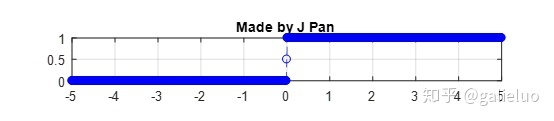
\includegraphics[width=0.6\textwidth]{figs/heaviside-func.png}
  \caption{figs:heaviside-func}
  \label{figs:heaviside-func}
\end{figure}

  我们现在说赫维赛德,当然不是因为这个函数,而是因为我们叹为观止、惊为天人、怎么夸都不过分的麦克斯韦方程组,麦克斯韦本人并没有见过这个方程组,它在一定程度上应该叫“赫维赛德方程组”。
\begin{equation}
  \begin{aligned}
    &{\Delta}{\cdot}D=\rho_{V}\\
    &{\Delta}{\cdot}B=0\\
    &{\Delta}{\times}E=-\frac{{\partial}B}{{\partial}t}\\
    &{\Delta}{\times}H=\frac{{\partial}D}{{\partial}t}+J
  \end{aligned}
\end{equation}

  这四个公式简直太对称了!而且它们的含义也很清晰:变化的电场产生磁场,变化的磁场产生电场,电磁波也就是电场和磁场此消彼长、相互转化、向前传播的形式。多亏了赫维赛德,麦克斯韦的理论才得以在十九世纪结束之前就真正站稳了脚跟并发扬光大。可以毫不谦虚地说:宇宙间任何的电磁现象,皆可由麦克斯韦方程组解释,包括光。也正是因为这个方程组完美统一了整个电磁场,让爱因斯坦始终想要以同样的方式统一引力场,并将宏观与微观的两种力放在同一组式子中,即著名的“大一统理论”。不幸的是麦克斯韦成功了,而爱因斯坦没有。

  麦克斯韦早在1873年便出版了跨时代巨著《电磁通论》,可惜的是,他英年早逝,他的方程组在生前并没有得到科学界的关注,其中一个很重要的原因是他的理论描述复杂得令人吃惊,他最初提出的电磁理论公式包含了二十个方程,直接导致他的理论在首次发表后的10多年时间内,几乎无人问津。

  赫维赛德最伟大的贡献是简化了麦克斯韦的原始方程组,通过他天才般的洞察力,挖掘出了蕴含在麦克斯韦方程式内部的深刻含义,从而使简化后的麦克斯韦方程组呈现出无与伦比的对称性,成为历史上最漂亮的方程式(没有之一)。

  而我们今天要说的,是赫维赛德的第二个重要贡献:运算微积分。学过电磁学的人都知道,在历史上人们发现的很多定理公式,都是用微积分的形式表达的。1880年-1887年之间,赫维赛德在从事电磁场研究的同时,为求解微积分方程,在他的分析计算中引入了微分算子的概念。它可以将常微分方程(ode)转换为普通代数方程。天才与普通人的区别就是人家靠“直觉”来解决问题的。赫维赛德是怎么解微分方程的呢?他把微分、积分运算用一个简单的算子来代替:
\begin{equation}
  \begin{aligned}
    &p{\leftrightarrow}\frac{d()}{dx}\\
    &p^{n}{\leftrightarrow}\frac{d^{n}()}{dx^{n}}\\
    &\frac{1}{p}{\leftrightarrow}\int_{-\infty}^{t}()d{\tau}
  \end{aligned}
\end{equation}

  也就是说,在某种算子下,积分和微分对应的是倒数关系,至于算子$p$代表什么,赫维赛德也没有多解释。在缺乏严密数学基础的情况下,人家直接放在文章里用了,还发表了。比如一个常见的二阶常微分方程:
\begin{equation}
  m\frac{d^{2}x}{dt}+c\frac{dx}{dt}+kx=0
\end{equation}
用赫维赛德的微分算子变换一下,就变成了代数表达式:
\begin{equation}
  mp^{2}+cp+k=0
\end{equation}

  赫维赛德之所以这么做,是因为他的“物理直觉”告诉他这么做,就是这么硬。这显然是一种开外挂的行为,因此也受到当时的主流科学家们的攻讦,他们认为赫维赛德就是十足的“民科”,文章没什么理论依据,自己在那空想呢。当然,赫维赛德也不是弱鸡,科学家怼起人来,也是毫不含糊:“因为我不能理解消化的过程就拒绝晚餐吗?不,只要我满意这个结果。”

  好了,扯了那么远,这些和拉普拉斯变换有什么关系?谜底就是:赫维赛德的微积分算子,就是拉普拉斯变换的前身。

  赫维赛德的算子验算虽然缺乏严密的数学基础,往往能给出重要且正确的结果,方法确实有效,无法驳倒。于是,在世纪之交,数学家们开始尝试对算子理论进行严格化。后来,人们在70年前法国数学家拉普拉斯的一本有关概率论的著作上,找到了这种算法的依据,但是这本书上提出的并不是现在我们看到的拉普拉斯变换,而是著名的Z变换。什么?拉普拉斯变换不是拉普拉斯提出的?随着二战后拉普拉斯变换的广泛使用,赫维赛德算子的作用被弱化了。但是不可否认的是,正是这种“不正规”,仅靠“天才的直觉”而发明的方法,促成了现在拉普拉斯分析法。

\section{傅里叶变换(轻量版拉普拉斯变换)}
  在说拉普拉斯变换以前,我们要先提一下傅里叶变换,这可以看成是轻量版的拉普拉斯变换。傅里叶变换说的是什么事?说的是自然界的很多现象,都可以用三角函数进行分解。
\begin{figure}[!htb]
  \centering
  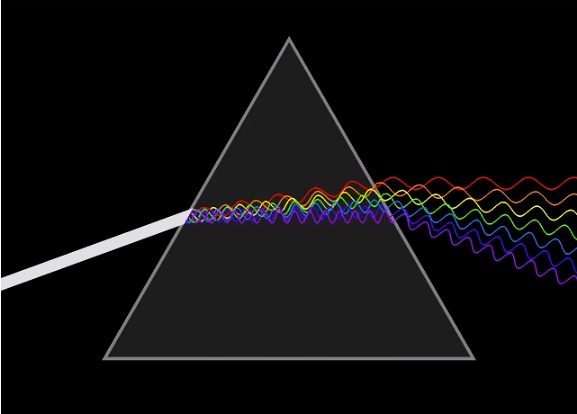
\includegraphics[width=0.4\textwidth]{figs/fourier-decomp.png}
  \caption{figs:fourier-decomp}
  \label{figs:fourier-decomp}
\end{figure}

  古巴比伦科学家在很早就使用了三角函数和逼近的方法,对天体运动进行观测和预报。1748年,大神欧拉用类似的方法分析弦的振动,1753年伯努利提出任意物理弦的振动都可以表达为三角函数的和,但是他没有给出证明(注意,伯努利是一个家族,3代人中产生了8位科学家,后裔有不少于120位被人们系统地追溯过)。1807年,傅里叶在法国科学学会上提交了一篇论文,运用正弦函数来描述温度分布,论文里有个在当时具有争议性的观点:任何连续周期信号都可以由一组适当的正弦函数组合而成。傅里叶没有做出严格的数学论证。这篇论文的审稿人中,有历史上著名的数学家拉格朗日和拉普拉斯,当拉普拉斯和其它审稿人通票通过并要发表这篇论文时,拉格朗日坚决反对,认为傅里叶的方法无法表示带有棱角的信号。法国科学学会屈服于拉格朗日的威望,拒绝了傅里叶的工作。1822年,傅里叶变换随其著作《热的解析》发表,但已经是15年之后了。1829年,狄利赫里通过推导其适用范围,完善了傅里叶变换。

\begin{figure}[!htb]
  \centering
  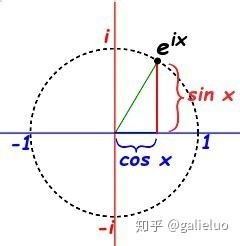
\includegraphics[width=0.3\textwidth]{figs/euler-func.png}
  \caption{figs:euler-func}
  \label{figs:euler-func}
\end{figure}
  我们知道,三角函数可以通过欧拉公式与复指数函数联系起来:
\begin{equation}
  e^{i{\omega}t}=\mathrm{cos}({\omega}t)+i\mathrm{sin}({\omega}t)
\end{equation}

  也就是说,复指数函数是与正弦函数、余弦函数紧密相关的,那是不是某些信号也能通过复指数函数进行分解呢?我们不妨先来研究一下$e^{i{\omega}t}$有什么特殊的性质。在这三篇文章\cite{fourier-transform-secret,nature-e-engineer-1,euler-formula}中,我们得出了以下结论:自然常数$e$可以描述事物的连续变化,虚数单位$i=\sqrt{-1}=e^{i\frac{\pi}{2}}$可以旋转,复指数函数$e^{i{\omega}t}$代表一个连续旋转的圆。

  因此,\{$e^{i{\omega}t}$\}可以看成时一组连续旋转的曲线,幅值永远为1,频率一直在变。这些旋转的曲线能做什么?
\begin{figure}[!htb]
  \centering
  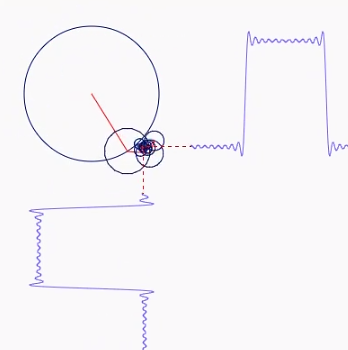
\includegraphics[width=0.4\textwidth]{figs/fourier-transform-example.png}
  \caption{figs:fourier-transform-example}
  \label{figs:fourier-transform-example}
\end{figure}

  你能想到很多曲线,都可以用这些不同频率、连续旋转的圆,通过线性叠加得到,而傅里叶定律,就是对这个结论的数学描述:只要一个函数满足狄利赫里条件,都能分解为复指数函数之和,哪怕是拉格朗日提到的带有棱角的方波函数。狄利赫里条件为:
\begin{enumerate}
  \item 函数在任意有限区间内连续,或只有有限个第一类间断点。
  \item 在一个周期内,函数有有限个极大值或极小值。
  \item $x(t)$绝对可积,即$\int_{0}^{\infty}\left|x(t)\right|\prec\infty$。
\end{enumerate}

  当满足狄利赫里条件时,傅里叶变换及其逆变换为:
\begin{equation}
  \begin{aligned}
    &F(\omega)=\int_{-\infty}^{+\infty}f(t)e^{-i{\omega}t}dt\\
    &f(t)=\frac{1}{2\pi}\int_{-\infty}^{+\infty}F(\omega)e^{i{\omega}t}d\omega
  \end{aligned}
\end{equation}

  于是就可以很好地解释拉格朗日和傅里叶之间的争论了,拉格朗日是对的:正弦曲线无法组合成一个带有棱角的信号,棱角处会有很小的高频波动(吉布斯现象)。但是,我们可以用正弦曲线来非常逼近地表示它,逼近到两种表示方法不存在能量差别。基于此,傅里叶也是对的。一个从数学家的角度,一个从工程师的角度。

\section{拉普拉斯变换(原来就是那么回事)}
  傅里叶变换能帮我们解决很多问题,一经问世后便受到广大工程师们的喜爱。因为它给人们提供了一扇不同的窗户来观察世界,从这个窗户来看,很多事情往往变得简单多了。但是,别忘了,傅里叶变换有一个很大的局限性,那就是信号必须满足狄利赫里条件才行,特别是那个绝对可积的条件,一下子就拦截掉了一大批函数。比如函数$f(t)=t^{2}$就无法进行傅里叶变换。这点难度当然难不到聪明的科学家,他们想到了一个绝佳的主意:把不满足绝对可积的函数乘以一个快速衰减的函数,这样在趋于$\infty$时原函数也衰减到零了,从而满足绝对可积。
\begin{figure}[!htb]
  \centering
  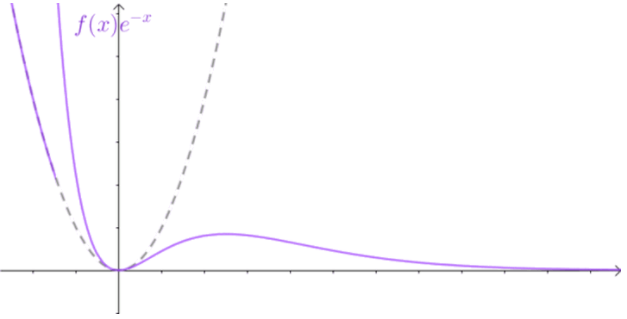
\includegraphics[width=0.6\textwidth]{figs/absolute-integrable.png}
  \caption{figs:absolute-integrable}
  \label{figs:absolute-integrable}
\end{figure}

  数学描述是:
\begin{equation}
  \lim_{x{\to}+{\infty}}f(x)e^{-{\sigma}x}=0,{\sigma}{\in}{\mathbb{R}}
\end{equation}
为保证$e^{-{\sigma}x}$一直为衰减函数,我们把$x$定义域缩减到正半轴,这样可以进行傅里叶变换就变成了:
\begin{equation}
  F({\omega})={\int}_{0}^{+\infty}f(t)e^{-{\sigma}t}e^{-i{\omega}t}dt=\int_{0}^{+\infty}f(t)e^{-({\sigma}+i{\omega})t}dt
\end{equation}
如果假设:
\begin{equation}
  s={\sigma}+i{\omega}
\end{equation}
那么就得到:
\begin{equation}
  F(s)=\int_{0}^{+\infty}f(t)e^{-st}dt
\end{equation}
这就是拉普拉斯变换。

  我知道大部分人前面的数学推导没什么兴趣,接下来就是放彩蛋的时刻了。之前提到的三篇文章\cite{fourier-transform-secret,nature-e-engineer-1,euler-formula}中说,$e^{i{\omega}t}$代表按不同频率旋转的单位圆,那是在复平面来看的。如果把时间轴也加上,$e^{i{\omega}t}$长什么样子呢?那就是螺旋曲线!从其他不同的平面看,螺旋曲线就是正弦或者余弦曲线。
\begin{figure}[!htb]
  \centering
  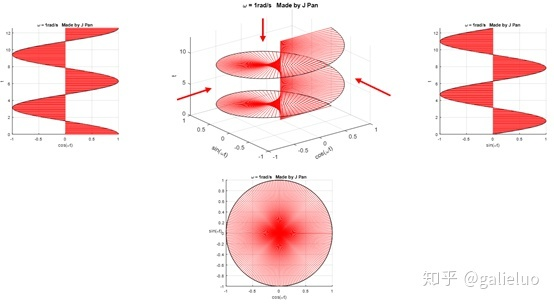
\includegraphics[width=0.6\textwidth]{figs/laplace-func-1.png}
  \caption{figs:laplace-func-1}
  \label{figs:laplace-func-1}
\end{figure}

  下面我们再来看看$e^{st},s=({\sigma}+i{\omega})$长什么样子。螺旋曲线和衰减函数的乘积:一个不断减小的螺旋曲线。从不同的平面看,就是不断衰减的正弦或者余弦曲线,从复平面来看,是一个半径不断减小的圆。
\begin{figure}[!htb]
  \centering
  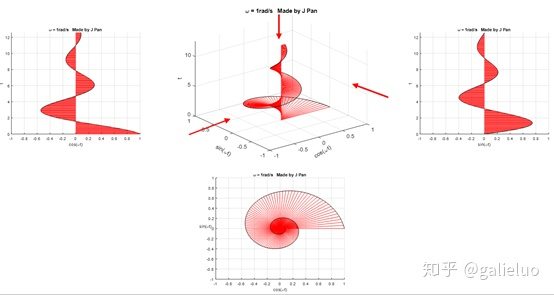
\includegraphics[width=0.6\textwidth]{figs/laplace-func-2.png}
  \caption{figs:laplace-func-2}
  \label{figs:laplace-func-2}
\end{figure}

\section{总结}
  傅里叶变换就是将函数分解到频率不同、幅值恒为1的单位圆上;拉普拉斯变换是将函数分解到频率幅值都在变化的圆上。因为拉普拉斯变换的基有了两个变量,因此更灵活,适用范围更广。

  最后的彩蛋:拉普拉斯变换和赫维赛德的微积分算子有什么关系?为什么说微分算子是拉普拉斯变换的前身?其实很简单。对于微分运算:$(e^{st})'=se^{st}$,令$f(t)=e^{st}$,则
\begin{equation}
  \frac{df(t)}{dt}=s{\cdot}f(t)
\end{equation}
对于积分运算:$\int_{-\infty}^{t}e^{s\tau}d\tau=\frac{1}{s}e^{st}$,令$f(t)=e^{st}$,则
\begin{equation}
  \int_{-\infty}^{t}f(\tau)d\tau=\frac{1}{s}f(t)
\end{equation}

  是不是和赫维赛德微分算子长得很像?

\nocite{*}
\bibliography{ref/refs}

\end{document}
